% Clase del documento
\documentclass[12pt,twoside,titlepage]{report}





%%%%%%%%%%%%%%%%%%%%%%% Paquetes %%%%%%%%%%%%%%%%%%%%%%%

\usepackage[a4paper,bindingoffset=3mm,bottom=35mm]{geometry}


% Usad \usepackage[dvips]{graphicx} o \usepackage[pdftex]{graphicx} (no ambos)
%\usepackage[dvips]{graphicx} %%% para LaTeX. Las figuras deben estar en formato eps

\usepackage[colorlinks=true,pdftex]{hyperref}   %%% Opcional. Para incluir marcadores y enlaces en el pdf
\usepackage[pdftex]{graphicx}  %%% para pdflatex. Las figuras pueden estar en pdf, jpg, svg y otros formatos


\usepackage[spanish]{babel}

%\usepackage[latin1]{inputenc} % Usad en WinEdt/MikTex
\usepackage[utf8]{inputenc} % Usad en overleaf

%\usepackage[T1]{fontenc}


% Algunos paquetes útiles

\usepackage{amsmath,amssymb}
\usepackage{hyperref}
\usepackage{color}
\usepackage{afterpage}
\usepackage{paralist}
\usepackage{array}
\usepackage{enumerate}
\usepackage{paralist}
\usepackage{enumitem}
\usepackage{float}
\usepackage{setspace}
\usepackage{listings}
\usepackage{algorithm}
\usepackage{algorithmic}
\usepackage{fancyhdr}
\usepackage{rotating}
\usepackage{multirow}


% Otros paquetes

\usepackage{quotchap}
\usepackage{lipsum}

%%%%%%%%%%%%%%%%%%%%%%%%%%%%%%%%%%%%%%%%%%%%%%%%%%%%%%%%






%%%%%%%%%%%%%%%%%%%%%%% Definiciones básicas %%%%%%%%%%%%%%%%%%%%%%%

\newcommand{\nombreautor}{Cristina Lozano Bautista}
\newcommand{\nombretutor}{Aaron Sujar}
\newcommand{\titulotrabajo}{Título del Trabajo de Fin de Grado}
\newcommand{\escuela}{Escuela Técnica Superior\\de Ingeniería Informática}
\newcommand{\escuelalargo}{Escuela Técnica Superior de Ingeniería Informática}
\newcommand{\universidad}{Universidad Rey Juan Carlos}
\newcommand{\fecha}{Junio de 2026}
\newcommand{\grado}{Grado en XXXXXXXX}
\newcommand{\curso}{Curso 20XX-20XX}
\newcommand{\logoUniversidad}{logoURJC.pdf} % logoURJC.eps

%%%%%%%%%%%%%%%%%%%%%%%%%%%%%%%%%%%%%%%%%%%%%%%%%%%%%%%%%%%%%%%%%%%%






%%%%%%%%%%%%%%%%%%%%%%%%% Otras definiciones %%%%%%%%%%%%%%%%%%%%%%%%%%

% Definiciones de colores (para hidelinks)
\definecolor{BlueLink}{rgb}{0.165,0.322,0.745}
\definecolor{PinkLink}{rgb}{0.8,0.22,0.5}
\definecolor{gray}{rgb}{0.6,0.6,0.6}


% Enlaces
\hypersetup{hidelinks,pageanchor=true,colorlinks,citecolor=PinkLink,urlcolor=black,linkcolor=BlueLink}


\newcommand\blankpage{%
    \newpage
    \null
    \thispagestyle{empty}%
    %\addtocounter{page}{-1}%
    \newpage}


% Texto referencias
\addto{\captionsspanish}{\renewcommand{\bibname}{Bibliografía}}

% Texto Índice de tablas
\addto\captionsspanish{
\def\tablename{Tabla}
\def\listtablename{\'{I}ndice de tablas}
}


\floatname{algorithm}{Algoritmo}

\newfloat{algorithm}{t}{lop}


%\newenvironment{pseudocodigo}[1][htb]
%  {\renewcommand{\algorithmcfname}{Pseudocódig}% Update algorithm name
%   \begin{algorithm}[#1]%
%  }{\end{algorithm}}
  
%%%%%%%%%%%%%%%%%%%%%%%%%%%%%%%%%%%%%%%%%%%%%%%%%%%%%%%%%%%%%%%%%%%%





%%%%%%%%%%%%%%%%%%%%%%% Estilo de código (en Python) %%%%%%%%%%%%%%%%%%%%%%%

\definecolor{bg}{rgb}{0.95,0.95,0.95}
\definecolor{mydeepteal}{rgb}{0.16,0.22,0.23}
\definecolor{myteal}{rgb}{0.31,0.44,0.46}
\definecolor{mymediumteal}{rgb}{0.41,0.58,0.60}

\DeclareFixedFont{\ttb}{T1}{txtt}{bx}{n}{12} % for bold
\DeclareFixedFont{\ttm}{T1}{txtt}{m}{n}{12}  % for normal


%\newcommand*{\FormatDigit}[1]{\textcolor{mydeepteal}{#1}}
\newcommand*{\FormatDigit}[1]{\textcolor{black}{#1}}

% Python style for highlighting
\newcommand\mypythonstyle{\lstset{
language=Python,
basicstyle=\ttfamily\small,
%basicstyle=\linespread{1.0}\footnotesize\ttm,
otherkeywords={self},             % Add keywords here
keywordstyle=\bfseries\ttfamily\color{myteal},
%keywordstyle=\ttb\color{myteal},
commentstyle=\itshape\color{myteal},
stringstyle=\color{mydeepteal},
emph={MyClass,__init__},          % Custom highlighting
emphstyle=\ttb\color{mydeepteal},    % Custom highlighting style
% Any extra options here
showstringspaces=false,            %
backgroundcolor=\color{bg},
rulecolor = \color{bg},
%identifierstyle=\color{deepgreen},
breaklines=true,
numbers=left,
numbersep=5pt,
numberstyle=\tiny,
tabsize=4,
xleftmargin=1em,
frame = single,
framesep = 3pt,
framextopmargin=0pt,
framexbottommargin=0pt,
framexleftmargin=0pt,
framexrightmargin=0pt,
fontadjust=true,
basewidth=0.55em, % compactness of code
upquote=true,
}}

% Python environment
\lstnewenvironment{mypython}[1][]
{
\mypythonstyle
\lstset{#1}
}
{}

\newcommand\mypythonstylenormalinline{\lstset{
language=Python,
basicstyle=\ttfamily\normalsize,
%basicstyle=\linespread{1.0}\footnotesize\ttm,
otherkeywords={self},            % Add keywords here
keywordstyle=\bfseries\ttfamily\color{myteal},
%keywordstyle=\ttb\color{myteal},
commentstyle=\itshape\color{mymediumteal},
stringstyle=\color{mydeepteal},
emph={MyClass,__init__},          % Custom highlighting
emphstyle=\ttb\color{mydeepteal},    % Custom highlighting style
% Any extra options here
showstringspaces=false,            %
backgroundcolor=\color{bg},
rulecolor = \color{bg},
%identifierstyle=\color{deepgreen},
breaklines=false,
numbers=left,
numbersep=5pt,
numberstyle=\tiny,
tabsize=4,
xleftmargin=0em,
frame = single,
framesep = 3pt,
framextopmargin=0pt,
framexbottommargin=0pt,
framexleftmargin=0pt,
framexrightmargin=0pt,
fontadjust=true,
%basewidth=0.55em, % compactness of code
upquote=true,
}}

\newcommand\mypythoninline[1]{{\mypythonstylenormalinline\lstinline!#1!}}

%%%%%%%%%%%%%%%%%%%%%%%%%%%%%%%%%%%%%%%%%%%%%%%%%%%%%%%%%%%%%%%%%%%%%%%%%%%%%%




%%%%%%%%%%%%%%%%%%%%%%%%%%%% Comandos definidos por el autor 

\newcommand{\transpuesta}{\mbox{\tiny $\mathsf{T}$}}








%%%%%%%%%%%%%%%%%%%%%%%%%%%%%%%%%%%%%%%%%%%%%%%%%%%%%%%%%%%%%%%%%%%%%%%
%                           Inicio del documento                       
%%%%%%%%%%%%%%%%%%%%%%%%%%%%%%%%%%%%%%%%%%%%%%%%%%%%%%%%%%%%%%%%%%%%%%%


\begin{document}

\pagestyle{plain}




%%%%%%%%%%%%%%%%%%%%%%%%%%%%%%%%%%%% Portada %%%%%%%%%%%%%%%%%%%%%%%%%%%%%%%%%%

%\pagenumbering{gobble}
%\pagenumbering{arabic}

% Universidad, Facultad
\begin{titlepage}
\selectlanguage{spanish}


% logo
\begin{center}
    \includegraphics[scale=0.7]{\logoUniversidad}
\end{center}

\bigskip

\begin{center}
\begin{LARGE}
\escuela \\
\end{LARGE}
\end{center}

\bigskip
\bigskip

% Grado
\begin{center}
\begin{large}
\textbf{\grado}\\
\end{large}
\end{center}

% Curso
\begin{center}
\begin{large}
\textbf{\curso}\\
\end{large}
\end{center}

\bigskip

\textbf{\begin{center}
\begin{large}
\textbf{Trabajo Fin de Grado}
\end{large}
\end{center}}

\bigskip
\bigskip
\bigskip

% Nombre del TFG
\begin{center}
\textbf{\begin{large}
\MakeUppercase{\titulotrabajo}\\
\end{large}}
\end{center}

% Nombre del autor
\vspace{\fill}
\begin{center}
\textbf{Autor: \nombreautor}\\ \smallskip
% Tutor
\textbf{Tutor: \nombretutor}\\
% Añadir segundo tutor si hubiera


\bigskip

% Fecha
%\textbf{\fecha}\\
\end{center}
\end{titlepage}


%%%%%%%%%%%%%%%%%%%%%%%% Opcional %%%%%%%%%%%%%%%%%%%%%%
%\blankpage

%\thispagestyle{empty}
%\begin{center}

% Nombre del trabajo
%\textbf{\begin{large}
%\MakeUppercase{\titulotrabajo}\\*
%\end{large}}
%\vspace*{0.2cm}
%\vspace{5cm}

% Nombre del autor y del tutor
%\large Autor: \nombreautor \\* \medskip
%\large Tutor: \nombretutor \\*

%\vfill

% Escuela, universidad y fecha
%\escuelalargo \\ \smallskip
%\universidad \\
%\vspace{1cm}
%\fecha \\

%\clearpage

%\end{center}
%%%%%%%%%%%%%%%%%%%%%%%%%%%%%%%%%%%%%%%%%%%%%%%%%%%%%%%%

\hypersetup{pageanchor=true}

\normalsize
\afterpage{\blankpage} % Se deben añadir página en blanco para que lo capítulos de la memoria o estas secciones introductorias empiecen en páginas impares

%%%%%%%%%%%%%%%%%%%%%%%%%%%%%%%%%%%%%%%%%%%%%%%%%%%%%%%%%%%%%%%%%%%%%%%%%%%%%%%





% Estilo de párrafo de los capítulos
\setlength{\parskip}{0.75em}
\renewcommand{\baselinestretch}{1.25}
% Interlineado simple
\spacing{1}

\pagenumbering{Roman}
\setcounter{page}{2}


%%%%%%%%%%%%%%%%%%%%%%%%% Agradecimientos o dedicatoria %%%%%%%%%%%%%%%%%%%%%%%%%%%

\chapter*{Agradecimientos}

Breves agradecimientos o dedicatoria.

\afterpage{\blankpage}

%%%%%%%%%%%%%%%%%%%%%%%%%%%%%%%%%%%%%%%%%%%%%%%%%%%%%%%%%%%%%%%%%%%%%%%%%%%%%%%%%%%






%%%%%%%%%%%%%%%%%%%%%%%%%%%%%%%%%%%% Resumen %%%%%%%%%%%%%%%%%%%%%%%%%%%%%%%%%%%%%%

\chapter*{Resumen}

La evaluación del pensamiento divergente mediante instrumentos como los Tests de Torrance (TTCT) suele realizarse en contextos de examen que el propio carácter evaluativo puede condicionar. Este Trabajo Fin de Grado presenta \textit{Sprout}, un prototipo de videojuego narrativo en el que la jugadora regenta una floristería en un pequeño pueblo y conversa con cuatro personajes gobernados por un modelo de lenguaje a gran escala. Mientras conversa con naturalidad, el juego estima de forma implícita cuatro dimensiones del pensamiento divergente inspiradas en las subpruebas verbales del TTCT ---fluidez, flexibilidad, originalidad y elaboración---, sin que la jugadora perciba contexto evaluativo alguno.

El sistema se sustenta sobre una arquitectura en capas con un dominio de lógica pura, independiente del motor, y sobre una herramienta propia: un editor visual de grafos de diálogo construido sobre la API GraphView del editor de Unity, que constituye el eje técnico del proyecto. El modelo de lenguaje desempeña un triple papel ---generación de diálogo en personaje, clasificación de la intención del jugador y evaluación de las ideas---, y las medidas resultantes se materializan en mecánicas jugables (flores emocionales, cotilleo nocturno y finales múltiples) en lugar de mostrarse como puntuaciones numéricas.

El alcance del trabajo es el de un prototipo funcional: se documenta el comportamiento del sistema, pero su validación psicométrica queda explícitamente fuera de alcance y se plantea como principal línea de trabajo futuro. La memoria detalla el diseño, la implementación técnica y la evaluación de usabilidad y experiencia del prototipo.

\mbox{} \bigskip

\noindent \textbf{Palabras clave}:
\begin{compactitem}
    \item Pensamiento divergente
    \item Tests de Torrance (TTCT)
    \item IA conversacional
    \item Modelos de lenguaje a gran escala (LLM)
    \item Videojuego narrativo
    \item Evaluación implícita
\end{compactitem}

\afterpage{\blankpage}

%%%%%%%%%%%%%%%%%%%%%%%%%%%%%%%%%%%%%%%%%%%%%%%%%%%%%%%%%%%%%%%%%%%%%%%%%%%%%%%%%%%





%%%%%%%%%%%%%%%%%%%%%%%%%%%%%%%%%%%% Índices %%%%%%%%%%%%%%%%%%%%%%%%%%%%%%%%%%%%

% Estilo de párrafo de los Índices
\setlength{\parskip}{1pt}
\renewcommand{\baselinestretch}{1}
\renewcommand{\contentsname}{Índice de contenidos}


% Índice de contenidos
\tableofcontents
\afterpage{\blankpage}

% Índice de tablas (OPCIONAL)
\listoftables
\afterpage{\blankpage}
\addcontentsline{toc}{chapter}{\noindent \listtablename}

% Índice de figuras (OPCIONAL)
\listoffigures
\afterpage{\blankpage}
\addcontentsline{toc}{chapter}{\listfigurename}

% Índice de códigos/algoritmos (OPCIONAL).   El término "Códigos" se puede cambiar por "Métodos", "Funciones", "Algoritmos", etc.
\renewcommand\lstlistlistingname{Códigos}
\renewcommand\lstlistingname{Código}
\renewcommand\lstlistlistingname{Índice de códigos}

\lstlistoflistings
\afterpage{\blankpage}
\addcontentsline{toc}{chapter}{\lstlistlistingname}


% En este documento (de momento) no se ha considerado incluir un índice de algoritmos/pseudocódigos, como el que aparece en \ref{AdditionalLouvain}

%%%%%%%%%%%%%%%%%%%%%%%%%%%%%%%%%%%%%%%%%%%%%%%%%%%%%%%%%%%%%%%%%%%%%%%%%%%%%%%%%%%





%%%%%%%%%%%%%%%%%%%%%%% Cabeceras y pies de página (Opcional) %%%%%%%%%%%%%%%%%%%%%%%

%\setlength{\headheight}{15.2pt}
\pagestyle{fancy}


\renewcommand{\chaptermark}[1]{\markboth{Capítulo \thechapter.\ #1}{}}

\pagestyle{fancy}
\fancyhf{}
\fancyhead[LO]{\leftmark}
\fancyhead[RO]{}
\fancyhead[RE]{\nouppercase\rightmark}
\fancyhead[LE]{}
\fancyfoot[C]{\thepage}

%%%%%%%%%%%%%%%%%%%%%%%%%%%%%%%%%%%%%%%%%%%%%%%%%%%%%%%%%%%%%%%%%%%%%%%%%%%%%%%%%%%%






%%%%%%%%%%%%%%%%%%%%%%%%%%%%%% Capítulos de la memoria %%%%%%%%%%%%%%%%%%%%%%%%%%%%%



% Capítulo 1
\chapter{Introducción}


%%%%%%%%%%%%%%%%%%%%%%%%%%%%%%%%%%%%%%%%%%%%%%%%%%%%%%%%%%%%%%%%%%%%%%%%%%

% Estilo resto de páginas
\pagestyle{fancy}


% Estilo de párrafo de los capítulos
\setlength{\parskip}{0.75em}
\renewcommand{\baselinestretch}{1.25}
% Interlineado simple
\spacing{1}
% Numeración contenido
\pagenumbering{arabic}
\setcounter{page}{1}

%%%%%%%%%%%%%%%%%%%%%%%%%%%%%%%%%%%%%%%%%%%%%%%%%%%%%%%%%%%%%%%%%%%%%%%%%%



\section{Motivación}

Este Trabajo Fin de Grado nace de una pregunta que rara vez se hace en la intersección entre videojuegos e investigación psicológica: ¿puede un videojuego evaluar habilidades cognitivas sin que el jugador perciba que está siendo evaluado? La hipótesis de la que parte Sprout es que sí, y que el medio idóneo para hacerlo es una experiencia narrativa conversacional con personajes gobernados por inteligencia artificial. El motivo es estructural: el propio Torrance, creador del instrumento más utilizado para medir la creatividad, advertía ya en 1972 que la palabra ``test'' debía evitarse delante del participante para no inhibir las respuestas creativas. Sprout lleva ese principio hasta su consecuencia última: la evaluación no se disfraza de juego, es un juego.

\textcolor{gray}{\textit{[Desarrollar: por qué este TFG cruza tres campos; por qué la creatividad; por qué un videojuego; por qué LLMs; cerrar con motivación personal breve. Ver guia\_completa.md sección 1.1.]}}

\section{Objetivos}

\subsection{Objetivo general}

Diseñar e implementar un prototipo funcional de videojuego narrativo en Unity que evalúe de forma implícita el pensamiento divergente de la jugadora a través de conversaciones con personajes no jugadores gobernados por un modelo de lenguaje conversacional con memoria persistente, siguiendo el marco operativo de las subpruebas verbales del Torrance Tests of Creative Thinking (Torrance, 1966/1974).

\subsection{Objetivos específicos}

Implementar una arquitectura limpia en Unity, desacoplada mediante ScriptableObjects y un sistema de eventos.

Diseñar e implementar un sistema de diálogo ramificado con flags acumulables y prerequisite gates.

Integrar un LLM como motor conversacional, con memoria persistente y personalidad diferenciada para cada NPC.

Operacionalizar las cuatro dimensiones del pensamiento divergente (fluidez, flexibilidad, originalidad, elaboración) en interacciones conversacionales.

Implementar el mapeo entre las seis subpruebas verbales vigentes del TTCT y las tramas narrativas del juego.

Diseñar e implementar la mecánica diferencial de la floristería emocional como bucle decisión-emoción-consecuencia.

Realizar un playtesting con usuarios reales para evaluar usabilidad, experiencia y comportamiento descriptivo del sistema.

Dejar diseñada y documentada la línea de validación psicométrica como trabajo futuro prioritario.

\section{Estructura del documento}

El presente documento se organiza en seis capítulos. El Capítulo I introduce el proyecto, su motivación y sus objetivos. El Capítulo II revisa el estado del arte en cuatro frentes: videojuegos como herramienta de evaluación, creatividad divergente y su medición, IA conversacional aplicada a videojuegos, y narrativa ramificada con incomodidad social. El Capítulo III detalla el diseño del videojuego desde el concepto hasta la mecánica diferencial. El Capítulo IV cubre la implementación técnica completa. El Capítulo V documenta la evaluación del prototipo. El Capítulo VI presenta conclusiones, limitaciones reconocidas y líneas de trabajo futuro. Cierran el documento las referencias bibliográficas y los anexos.

\section{Plan de trabajo}

\textcolor{gray}{\textit{[Redactar al cierre del TFG con cronograma real, hitos, fases. Insertar diagrama de Gantt como figura.]}}

\chapter{Estado del arte}

El presente capítulo establece el marco teórico y referencial sobre el que se construye Sprout. Se estructura en cuatro frentes complementarios: el videojuego como herramienta de evaluación cognitiva y experiencia interactiva (2.1), la creatividad divergente y los instrumentos clásicos para evaluarla (2.2), la inteligencia artificial conversacional aplicada al medio videojuego (2.3) y la tradición de narrativa ramificada con incomodidad social, con especial atención al precedente de Façade (2.4). Cada sección presenta primero la idea principal, la ancla con referencias académicas, conecta el marco con decisiones específicas de diseño de Sprout y cierra explicitando una limitación o acotación de alcance.

\section{Videojuegos como herramienta de evaluación y experiencia interactiva}

Los videojuegos han transitado, en las últimas dos décadas, desde su consideración como mero entretenimiento de consumo hasta convertirse en herramientas legítimas de investigación cognitiva, intervención clínica y evaluación psicológica. Granic, Lobel y Engels (2014) sintetizaron en American Psychologist la evidencia acumulada sobre los beneficios cognitivos, motivacionales, emocionales y sociales del medio, abriendo formalmente el espacio académico para considerar al videojuego un vehículo de evaluación e intervención. Sprout se sitúa explícitamente en esa tradición, aunque con una acotación importante que se desarrolla al final de esta sección.

\textcolor{gray}{\textit{[Desarrollar: serious games, narrativa embebida (Jenkins 2004), Hamlet on the Holodeck (Murray 1997), transportación narrativa (Green \& Brock 2000). Cerrar con acotación: Sprout no es serious game terapéutico, es prototipo de evaluación implícita exploratoria.]}}

\section{Creatividad divergente y su evaluación}

Esta sección recorre el desarrollo histórico y técnico de la evaluación del pensamiento divergente desde sus orígenes con Guilford hasta el estado actual del Torrance Tests of Creative Thinking, pasando por sus dos formas (Figural y Verbal), sus métricas compuestas, su filosofía de aplicación no amenazante y las críticas a su validez. Cada subapartado conecta con decisiones específicas de diseño de Sprout.

\subsection{Origen: el pensamiento divergente de Guilford}

El concepto de pensamiento divergente como dimensión cognitiva diferenciada fue introducido por J. P. Guilford en su modelo estructural del intelecto (Guilford, 1967). A diferencia del pensamiento convergente ---orientado a encontrar la respuesta única correcta a un problema---, el divergente produce múltiples soluciones alternativas a partir de un mismo estímulo. Para operacionalizarlo, Guilford diseñó el Alternative Uses Task (AUT), una tarea en la que se pide al participante listar todos los usos posibles que se le ocurran para un objeto cotidiano en un tiempo limitado.

\textcolor{gray}{\textit{[Desarrollar: distinción convergente/divergente, ejemplo del ladrillo, las cuatro dimensiones canónicas (fluidez, flexibilidad, originalidad, elaboración) y su continuidad en Sprout.]}}

\subsection{Operacionalización: Torrance y el TTCT}

E. Paul Torrance recogió el marco de Guilford y lo desarrolló en una batería estandarizada de pruebas: los Torrance Tests of Creative Thinking (TTCT). Publicado originalmente en 1966 y revisado en sucesivas ediciones, el TTCT sigue siendo casi sesenta años después el instrumento más utilizado y validado para la evaluación del pensamiento divergente (Kim, 2006; Acar \& Runco, 2022). Se distribuye en dos formas paralelas, Figural y Verbal, cada una con dos versiones equivalentes (A y B) que permiten mediciones pre y post sin contaminación de aprendizaje.

\textcolor{gray}{\textit{[Desarrollar: quién es Torrance, las dos formas, las dos versiones, distribución comercial por STS.]}}

\subsection{Las subpruebas verbales del TTCT}

La forma verbal del TTCT consta actualmente de seis actividades, tras la eliminación de la histórica Unusual Questions por considerarse redundante en la literatura más reciente (Acar \& Runco, 2022). Las seis vigentes son: Asking Questions, Guessing Causes, Guessing Consequences, Product Improvement, Unusual Uses y Just Suppose. Cada actividad se puntúa en tres dimensiones norm-referenced: fluidez, flexibilidad y originalidad. A diferencia de la forma figural, la verbal no incorpora dimensiones como abstracción de títulos o resistencia al cierre prematuro, que son específicas del medio gráfico.

Es importante destacar que las formas Verbal y Figural del TTCT no miden las mismas habilidades creativas. Aunque dos dimensiones se evalúan en ambos formatos (fluidez y originalidad), el rendimiento entre ellas correlaciona muy poco. Cramond (1994) reportó una correlación de r = 0.06 entre originalidad verbal y figural. El hallazgo se replicó en Ulger (2015), que con una muestra de estudiantes turcos de séptimo grado obtuvo una correlación débil entre originalidad figural y verbal (r = 0.18, p = 0.06) y una correlación moderada para fluidez (r = 0.33, p < 0.05). Estos datos confirman que la forma verbal y la figural del TTCT miden constructos parcialmente independientes.

Sprout implementa exclusivamente las subpruebas verbales del TTCT. Esta acotación no compromete el rigor del marco teórico sino que define un alcance metodológicamente coherente: dado que verbal y figural miden habilidades parcialmente independientes (Cramond, 1994; Ulger, 2015), cubrir la forma verbal de manera completa es una decisión legítima de alcance, no una omisión. La implementación de subpruebas figurales mediante una mecánica de dibujo se contempla como línea de trabajo futuro (Cap. VI).

\textcolor{gray}{\textit{[Desarrollar: describir las seis actividades con ejemplo de estímulo. Anticipar el mapeo a tramas y personajes (detallado en Cap. III sección 3.3): tres plenamente (Product Improvement con Aster, Unusual Uses con Mochi, Just Suppose con Moth) y tres integradas de forma ligera.]}}

\subsection{Filosofía de aplicación no amenazante}

Uno de los aspectos más relevantes del manual original del TTCT Figural (Torrance, 1972, pp. 4-6) es la prescripción explícita sobre cómo debe administrarse el test. Torrance argumenta que la palabra ``test'' no debe utilizarse delante de los participantes; los cuadernillos están deliberadamente titulados Thinking Creatively With Pictures, no Test of Creative Thinking. La atmósfera de la sesión debe ser lúdica, de juego y resolución de problemas, evitando la situación amenazante asociada a la evaluación. Torrance sostiene que un contexto evaluativo explícito inhibe las respuestas creativas y degrada la validez de la medición.

\textcolor{gray}{\textit{[Desarrollar: continuidad metodológica entre la prescripción de Torrance y la propuesta de evaluación implícita de Sprout. Esta es la justificación académica más fuerte del proyecto.]}}

\subsection{Fiabilidad de evaluadores no entrenados}

Un dato especialmente relevante para Sprout aparece en el manual del TTCT Figural en la sección sobre fiabilidad inter-evaluadora (Torrance, 1972, p. 10). Torrance reportó coeficientes de correlación Pearson de entre 0.86 y 0.96 entre evaluadores entrenados y evaluadores no entrenados (profesores de aula y secretarios educativos), siempre que estos siguieran estrictamente la guía de scoring del manual. La conclusión metodológica es que no es necesario entrenamiento especializado para alcanzar fiabilidad aceptable, sino la adopción rigurosa de los criterios operativos del manual.

\textcolor{gray}{\textit{[Desarrollar: el argumento clave de Sprout. Si un evaluador humano no entrenado alcanza r = 0.86-0.96 siguiendo guía, es razonable hipotetizar que un LLM con system prompt derivado del manual puede comportarse de forma análoga. Reconocer que es hipótesis y que validación rigurosa queda como trabajo futuro.]}}

\subsection{Crítica y vigencia del TTCT}

La referencia crítica más citada sobre el TTCT es Kim (2006), ``Can we trust creativity tests? A review of the Torrance Tests of Creative Thinking''. Kim revisa cuarenta años de evidencia sobre fiabilidad y validez del instrumento y concluye que, pese a las críticas acumuladas, el TTCT sigue siendo el instrumento más sólido disponible para evaluar pensamiento divergente. Para contexto hispanohablante, Almeida et al. (2008) examinaron la validez de constructo del TTCT en muestras españolas y portuguesas, y Krumm et al. analizaron la estructura factorial del TTCT Verbal Forma B en población hispanohablante.

\textcolor{gray}{\textit{[Desarrollar: síntesis de críticas, respuesta de Kim, datos hispanohablantes. Argumentar que citar las críticas demuestra rigor y no asunción acrítica.]}}

\subsection{Limitación y posicionamiento de Sprout}

A lo largo de esta sección 2.2 se ha presentado el marco operativo del que parte Sprout: el pensamiento divergente como dimensión cognitiva diferenciada (Guilford, 1967), el TTCT como instrumento estandarizado para evaluarlo (Torrance, 1966/1974/1972; STS, 2018), su filosofía de aplicación no amenazante (Torrance, 1972), la fiabilidad demostrada de evaluadores no entrenados con guía (Torrance, 1972) y la independencia parcial entre las formas verbal y figural (Cramond, 1994; Ulger, 2015). Sprout adopta este marco como referencia conceptual, no como instrumento a replicar. El sistema no pretende equivalencia psicométrica con el TTCT, sino proporcionar un indicador análogo derivado conceptualmente de su marco, implementado en un medio (conversación por voz con LLM) estructural y técnicamente distinto al medio original del TTCT (papel y lápiz con evaluador humano). Esta acotación se mantiene explícita a lo largo de toda la memoria.

\section{IA conversacional en videojuegos}

Esta sección recorre los fundamentos técnicos y conceptuales que permiten integrar IA conversacional con memoria persistente en un videojuego narrativo. Se cubren los modelos de lenguaje a gran escala, su uso como personajes con personalidad consistente, las técnicas de prompt engineering, la gestión de memoria persistente entre interacciones, el uso emergente de LLMs como evaluadores en tareas cognitivas y, finalmente, los límites éticos que Sprout asume.

\subsection{Modelos de lenguaje a gran escala (LLMs)}

Los modelos de lenguaje a gran escala basados en arquitecturas transformer representan el salto cualitativo que ha hecho posible la integración de IA conversacional en videojuegos como elemento de gameplay y no únicamente como herramienta de desarrollo. Brown et al. (2020) presentaron GPT-3 y demostraron la capacidad few-shot de los LLMs para realizar tareas no entrenadas explícitamente, lo que abrió el camino al uso de prompts como mecanismo de control del comportamiento del modelo. El informe técnico de GPT-4 (OpenAI, 2023) consolidó la capacidad de estos modelos para mantener conversaciones coherentes, asumir personalidades distintas y razonar sobre contextos complejos.

\textcolor{gray}{\textit{[Desarrollar: qué es un LLM, por qué los prompts importan, limitaciones (alucinaciones, sesgos, no determinismo, coste), justificación del modelo elegido en Sprout.]}}

\subsection{LLMs como personajes en videojuegos}

Bickmore y Picard (2005) anticiparon, antes incluso de la era de los LLMs modernos, los principios de diseño que rigen la relación a largo plazo entre humanos y agentes conversacionales. Su trabajo sobre relational agents establece que la confianza y la persistencia de la relación dependen de tres factores: la consistencia del personaje, su memoria de interacciones previas y su capacidad de adaptación al usuario. Estos tres principios se aplican directamente a los cuatro NPCs de Sprout ---Mochi, Aster, Moth y Rix---, cada uno con personalidad fija, voz diferenciada y memoria persistente.

\textcolor{gray}{\textit{[Desarrollar: los tres principios y su aplicación a Sprout. Mencionar contexto industrial actual (NVIDIA ACE, Inworld AI, demos de Ubisoft) si encaja.]}}

\subsection{Prompt engineering y system prompts}

El comportamiento de un LLM se modula principalmente a través del prompt que recibe como entrada. Wei et al. (2022) demostraron que la inclusión de cadenas de razonamiento explícitas en los prompts mejora significativamente el desempeño en tareas complejas, técnica conocida como Chain-of-Thought Prompting. Esta y otras técnicas relacionadas (in-context learning, role prompting, few-shot prompting) son las herramientas con las que se diseñan los system prompts dinámicos de Sprout, donde cada NPC recibe un prompt que combina su personalidad fija, su memoria persistente y el contexto narrativo del momento.

\textcolor{gray}{\textit{[Desarrollar: system prompt vs user prompt, técnicas de prompting, combinación de personalidad estática + memoria dinámica + contexto en Sprout.]}}

\subsection{Memoria persistente en agentes conversacionales}

La memoria persistente de los NPCs de Sprout se implementa mediante inyección de contexto: cada interacción se serializa, se almacena en disco, y los fragmentos relevantes se reinyectan en el prompt de interacciones posteriores. Esta técnica, distinta del fine-tuning del modelo base, permite que un NPC recuerde eventos pasados sin necesidad de reentrenar el LLM y manteniendo el coste computacional acotado.

\textcolor{gray}{\textit{[Desarrollar: diferencia inyección de contexto vs fine-tuning. Estrategias de selección de qué recordar. Documentar lo implementado, no lo aspiracional.]}}

\subsection{LLM como evaluador en tareas cognitivas}

El uso de LLMs como evaluadores automáticos de respuestas humanas es un campo emergente con literatura aún en consolidación. La hipótesis de fondo es que un LLM con guía operativa explícita puede puntuar respuestas con fiabilidad comparable a un evaluador humano no entrenado pero guiado, apoyándose en el precedente histórico ya citado de Torrance (1972) sobre fiabilidad de evaluadores no entrenados. Sprout opera bajo esta hipótesis y declara explícitamente que la validación rigurosa de la fiabilidad del LLM evaluador queda como trabajo futuro prioritario (Cap. VI).

\textcolor{gray}{\textit{[Desarrollar: usos actuales del LLM como juez, limitaciones, justificación de la decisión en Sprout.]}}

\subsection{Límites éticos}

La integración de IA conversacional en contextos donde se recogen respuestas cognitivas de los usuarios exige un posicionamiento ético claro y explícito. Sprout no es ---ni se presenta como--- herramienta terapéutica, herramienta de diagnóstico psicológico, ni instrumento de selección de personal. Es un prototipo de entretenimiento con un componente experimental de evaluación implícita, con fines exclusivamente de investigación y demostración técnica en el contexto de este TFG.

\textcolor{gray}{\textit{[Desarrollar: lista de lo que Sprout NO es. Mencionar Woebot Health como contraste (no como analogía). Tratar protección de datos: anonimización, consentimiento en playtesting.]}}

\section{Narrativa ramificada e incomodidad social en juegos conversacionales}

Façade (Mateas \& Stern, 2003) es la referencia académica fundacional para Sprout en su capa de incomodidad social. Façade es un drama interactivo en tiempo real donde el jugador entra en el apartamento de una pareja en crisis y mantiene conversaciones por texto natural. Los personajes pueden discutir entre ellos, ofenderse, sentirse manipulados y reaccionar emocionalmente a las palabras del jugador. Façade introdujo el concepto de tensión social emergente como motor narrativo, donde la incomodidad no es un fallo del diseño sino su rasgo distintivo. Sprout adopta esta tradición pero la combina deliberadamente con una capa estética opuesta: la calidez visual y emocional de juegos como Animal Crossing o Tomodachi Life. Esta tensión entre lo bonito y lo extraño es lo que define la identidad del juego.

\textcolor{gray}{\textit{[Desarrollar: descripción detallada de Façade, distinción tradición Inkle vs tradición Façade (Sprout es híbrido), referencia estética (Animal Crossing, Tomodachi) explícitamente como estética y NO como narrativa.]}}

\chapter{Diseño del videojuego}

Este capítulo detalla el diseño de Sprout: de la premisa al detalle de la mecánica diferencial. Se estructura siguiendo el camino que cualquier equipo de diseño recorre al definir un videojuego: primero el concepto y los pilares (3.1), después los espacios y el ritmo del juego (3.2), los personajes y su mapeo a las subpruebas del TTCT (3.3), la arquitectura narrativa ramificada (3.4), la operacionalización de la evaluación implícita (3.5), la mecánica diferencial de la floristería emocional (3.6) y, finalmente, las decisiones de diseño que requieren defensa explícita (3.7).

\section{Concepto y premisa}

Sprout es un videojuego narrativo de corta duración ---aproximadamente quince minutos por partida--- en el que la jugadora regenta una floristería en un pueblo pequeño habitado por cuatro vecinos. Cada partida representa un día completo en el pueblo, dividido en cuatro momentos: mañana, mediodía, tarde y noche. Durante el día, la jugadora conversa con los vecinos, ayuda con sus dilemas, decide qué decir y a quién, y combina flores para preparar ramos emocionales. Durante la noche, los vecinos conversan entre sí sin que la jugadora esté presente, propagando información a través del pueblo.

\textcolor{gray}{\textit{[Desarrollar: los tres pilares de diseño (creatividad como mecánica no métrica visible / incomodidad social como motor / sin puntuaciones visibles); duración corta como decisión deliberada; referencias Façade y Animal Crossing.]}}

\section{Diseño del pueblo y la floristería}

El espacio de juego de Sprout está deliberadamente acotado: un pueblo pequeño con la floristería como hub central y cuatro casas adyacentes pertenecientes a cada uno de los vecinos. Esta acotación responde tanto a restricciones técnicas del prototipo como a una decisión de diseño narrativo: un mundo pequeño concentra la atención emocional y permite que cada decisión tenga consecuencias visibles en personajes con los que la jugadora ha pasado tiempo.

\textcolor{gray}{\textit{[Desarrollar: floristería como hub, progresión del jardín como narrador, estructura del día en cuatro momentos. Insertar mapa del pueblo como figura.]}}

\section{Diseño de personajes y mapeo a subpruebas verbales del TTCT}

Sprout cuenta con cinco personajes: la protagonista (la florista) y cuatro vecinos ---Mochi, Aster, Moth y Rix---. Cada vecino tiene una personalidad fija, una voz diferenciada y una trama propia que se desarrolla a lo largo del día. La asignación de subpruebas del TTCT-Verbal a cada personaje no es arbitraria: se ha buscado que el rasgo dominante de cada personaje active de forma natural el tipo de pensamiento que esa subprueba evalúa.

\textcolor{gray}{\textit{[Desarrollar: la florista (lienzo), Mochi (Unusual Uses), Aster (Product Improvement), Moth (Just Suppose + Asking ligera), Rix (catalizador moral, Guessing Causes y Consequences ligeras).]}}

La siguiente tabla resume el mapeo entre subpruebas del TTCT-Verbal y momentos del juego:

\textcolor{gray}{\textit{[Justificar el reparto 3+3: viabilidad de prototipo, coherencia narrativa, cobertura conceptual completa, base para extensión futura.]}}

\section{Diseño de la narrativa ramificada}

La narrativa de Sprout se estructura como un grafo dirigido de nodos conversacionales, cada uno con condiciones de activación (prerequisite gates) basadas en flags acumulados durante la partida. Esta estructura es la heredera directa de la tradición de Inkle (80 Days, Heaven's Vault) y de Choice of Games, donde la agencia narrativa real se construye no con árboles binarios simples sino con redes de condiciones acumulables que generan caminos emergentes.

\textcolor{gray}{\textit{[Desarrollar: nodos y flags (insertar diagrama UML), las cuatro tramas en paralelo, sistema de cotilleo nocturno, finales múltiples. La implementación técnica va en Cap. IV.]}}

\section{Diseño de la evaluación implícita}

El núcleo distintivo de Sprout es su sistema de evaluación implícita: el juego mide pensamiento divergente sin que la jugadora perciba el contexto evaluativo. Esta sección detalla cómo se operacionalizan las cuatro dimensiones del TTCT-Verbal (fluidez, flexibilidad, originalidad y elaboración) en interacciones conversacionales, cómo se acumulan en un perfil de creatividad por personaje ---sin construir un índice compuesto normativo, que exigiría una calibración fuera del alcance de este trabajo--- y cómo se proporciona feedback a la jugadora sin recurrir nunca a puntuaciones numéricas visibles.

\textcolor{gray}{\textit{[Desarrollar: operacionalización dimensión por dimensión (fluidez y flexibilidad como conteos; originalidad y elaboración como medias normalizadas en [0,1]); cómo se acumulan en un perfil por NPC y un agregado para el final; mecanismo de feedback (frase narrativa + flor); justificación con remisión a 2.2.4. Nota: no se calcula un índice compuesto ni fortalezas creativas, pues requerirían calibración normativa fuera de alcance.]}}

\section{La floristería emocional: mecánica diferencial}

La mecánica diferencial de Sprout ---el rasgo que distingue al juego de cualquier otro proyecto similar--- es la floristería emocional. Cada noche, según las decisiones tomadas durante el día, brotan en el jardín de la florista flores con carga emocional asociada. Al día siguiente, la jugadora combina dos flores para crear ramos con nombre y significado propios, y los regala a los vecinos. El mismo ramo no significa lo mismo para todos los personajes: el sistema de reacciones diferenciales por NPC convierte cada regalo en una decisión narrativa con consecuencias específicas.

\textcolor{gray}{\textit{[Desarrollar: tabla de las siete flores base con emoción y comportamiento generador; tabla parcial de combinaciones (completa en Anexo E); reacciones diferenciales por NPC; justificación académica del bucle decisión-emoción-consecuencia.]}}

\section{Decisiones de diseño defendibles}

Algunas decisiones de diseño de Sprout requieren defensa explícita porque podrían ser cuestionadas en evaluación académica. Esta sección recoge las cinco más importantes y la justificación de cada una.

\textcolor{gray}{\textit{[Desarrollar cada decisión como un párrafo independiente: 1) conversación por voz vs texto; 2) cuatro NPCs; 3) 15 minutos por partida; 4) pruebas verbales y no figurales (USAR AQUÍ EL DATO Cramond 1994 / Ulger 2015); 5) tres subpruebas plenas + tres ligeras. Para cada decisión, declarar la contrapartida.]}}

\chapter{Implementación técnica}

Este capítulo describe la implementación técnica del prototipo Sprout en Unity 6. La arquitectura adopta principios de Clean Architecture (Martin, 2017) adaptados al entorno Unity (Nystrom, 2014; Hipple, 2017), con una separación clara entre lógica de dominio, lógica de aplicación, infraestructura y presentación. La comunicación entre módulos se realiza mediante un sistema de eventos basado en ScriptableObjects que mantiene los componentes desacoplados y testeables. El capítulo se organiza siguiendo las capas y módulos principales del sistema, desde la arquitectura general hasta el pipeline de renderizado.

\section{Arquitectura del sistema}

La arquitectura de Sprout se construye sobre el principio de inversión de dependencias: la lógica de dominio (reglas narrativas, estado del juego, evaluación implícita) no depende de detalles de infraestructura ni de presentación. Para conseguirlo en Unity, donde el ciclo de vida MonoBehaviour fuerza dependencias laterales, se ha recurrido a la combinación de ScriptableObjects como almacén de configuración y estado puro (Hipple, 2017), Assembly Definitions para imponer la regla de dependencias, e interfaces que abstraen las fronteras entre capas.

\textcolor{gray}{\textit{[Desarrollar: las cuatro capas (insertar diagrama UML), Assembly Definitions, SOs vs Singletons, interfaces (ISettingsRepository, ISceneLoader, IInteractable, IPlayerController).]}}

\section{Sistema de estados --- HFSM}

El estado del juego y del jugador se gestiona mediante una máquina de estados finitos jerárquica (HFSM) que separa flujos macro (del juego completo) y flujos micro (del personaje jugador). Esta separación, recomendada por Millington y Funge (2009), evita el anti-patrón de máquinas de estado planas con explosión combinatoria de transiciones.

\textcolor{gray}{\textit{[Desarrollar: GameStateMachine (Boot, MainMenu, Loading, Playing, Paused, Ending), PlayerStateMachine (FreeRoam, Dialogue, Inspect, Paused), NPCStateMachine. Diagramas de transiciones.]}}

\section{Sistema de diálogo ramificado y editor visual de grafos}

El sistema de diálogo constituye la columna vertebral de la interacción en Sprout: es el medio por el que la jugadora conversa con los personajes y, en consecuencia, el soporte sobre el que se asienta la evaluación implícita del pensamiento divergente. Por este motivo no se resolvió mediante texto codificado de forma rígida ni con un complemento de terceros, sino que se diseñó e implementó una herramienta propia: un editor visual de grafos de diálogo integrado en el editor de Unity. Esta sección documenta su motivación, su modelo de datos, el editor visual, el mecanismo de serialización, su ejecución en tiempo de juego y su integración con la inteligencia artificial.

\subsection{Motivación y enfoque general}

Una conversación con ramificaciones, condiciones de acceso y consecuencias narrativas puede representarse de forma natural como un grafo dirigido: cada nodo es un momento de la conversación y cada arista una posible continuación. Codificar este grafo a mano ---en estructuras de datos dentro del código fuente o en hojas de cálculo--- resulta propenso a errores y difícil de mantener conforme la narrativa crece. La alternativa de emplear un complemento comercial se descartó para conservar el control total sobre el modelo de datos y, sobre todo, para poder integrar de forma nativa el contexto que cada nodo aporta a la inteligencia artificial, requisito específico de este proyecto que las soluciones genéricas no contemplan.

Se optó, por tanto, por construir una herramienta a medida sobre \textbf{GraphView}, la API del editor de Unity para la edición de grafos. La herramienta permite diseñar conversaciones de manera visual ---creando cajas y trazando flechas entre ellas--- de modo que la persona responsable del diseño narrativo trabaja sobre una representación gráfica y no sobre código. El planteamiento sigue la separación de responsabilidades adoptada en todo el proyecto: por un lado, un modelo de datos que el juego ejecuta en tiempo real; por otro, un editor que vive exclusivamente en el entorno de desarrollo y que lee y escribe ese mismo modelo.

\subsection{Modelo de datos: el grafo y los nodos}

El grafo se representa mediante el ScriptableObject \texttt{DialogueGraphSO}, que almacena la lista de nodos que lo componen, una referencia al nodo de entrada y las posiciones de cada nodo en el lienzo del editor. El empleo de ScriptableObjects es deliberado: son el mecanismo de serialización propio de Unity y permiten que el contenido narrativo se gestione como un recurso del proyecto, independiente de las escenas.

Todos los nodos derivan de la clase abstracta \texttt{DialogueNodeSO}, que reúne los atributos comunes a cualquier momento de la conversación: un identificador único (\texttt{nodeGuid}), el contexto que se transmite a la inteligencia artificial en ese punto (\texttt{contextForAI}), las condiciones de acceso, los cambios de estado que se aplican al entrar, una respuesta alternativa para cuando no se cumplen los requisitos y la lista de nodos siguientes. Sobre esta base se definen tres tipos concretos de nodo, resumidos en la Tabla~\ref{tab:tipos_nodo}.

\begin{table}[h]
  \centering
  \caption{Tipos de nodo del sistema de diálogo.}
  \label{tab:tipos_nodo}
  \begin{footnotesize}
  \renewcommand{\arraystretch}{1.3}
  \begin{tabular}{p{2.6cm}p{6cm}p{4.5cm}}
    \hline
    \textbf{Tipo de nodo} & \textbf{Comportamiento} & \textbf{Campos propios} \\
    \hline
    SpeechNode & El NPC pronuncia una línea y la conversación avanza, de forma automática o según condiciones evaluadas por la IA. & Frase inicial; transiciones (condición y nodo destino). \\
    \hline
    ChoiceNode & Punto de ramificación explícita: la jugadora elige entre varias opciones y cada una conduce a un nodo distinto. & Frase inicial; lista de opciones, cada una con condición y nodo destino. \\
    \hline
    ConversationNode & Conversación abierta sobre varios temas dentro del mismo nodo; no se ramifica. Solo avanza cuando la IA determina que se cumple una condición de salida. & Frase inicial; temas de conversación; condición de salida. \\
    \hline
  \end{tabular}
  \end{footnotesize}
\end{table}

La distinción entre el ChoiceNode y el ConversationNode es la que mejor ilustra la filosofía del sistema. El ChoiceNode representa una ramificación cerrada y clásica: opciones discretas con destinos predefinidos. El ConversationNode, en cambio, habilita una conversación libre en lenguaje natural alrededor de unos temas sugeridos, en la que el avance no depende de una elección de menú sino de que la inteligencia artificial reconozca que se ha satisfecho una condición expresada en lenguaje natural. Esta dualidad permite combinar tramos de narrativa firmemente guionizados con tramos de diálogo abierto.

\subsection{Puertas narrativas y banderas de estado}

El control del progreso narrativo se realiza mediante banderas (flags) booleanas. Cada nodo puede declarar una lista de requisitos previos, donde cada requisito asocia el nombre de una bandera con el valor esperado. Antes de permitir el acceso a un nodo, el sistema comprueba que todas las banderas requeridas tengan el valor previsto; si no es así, el nodo permanece bloqueado y, opcionalmente, se devuelve una respuesta definida para ese caso. De manera complementaria, un nodo puede activar banderas al ser alcanzado, lo que permite que la historia registre que la jugadora ha pasado por un determinado momento y desbloquee, en consecuencia, contenidos posteriores. Este mecanismo convierte el grafo en una máquina narrativa con memoria de estado, cuyas banderas alimentan además el sistema de cotilleos nocturnos y la resolución del final.

\subsection{El editor visual basado en GraphView}

El editor se materializa en una ventana de editor accesible desde el menú de herramientas de Unity, que ofrece acciones para guardar y cargar grafos. El lienzo proporciona las manipulaciones habituales de un editor de grafos ---zoom, desplazamiento, rejilla de fondo y selección por rectángulo--- y responde a la petición de creación de nodos abriendo un buscador que permite insertar cualquiera de los tres tipos de nodo en la posición del cursor. Cada nodo se dibuja codificando su tipo por color ---azul para Speech, marrón para Choice y verde para Conversation---, lo que facilita la lectura del grafo de un vistazo. Dentro de cada caja se exponen, de forma editable en línea, los campos relevantes del nodo. Las conexiones se establecen a través de puertos: cada nodo dispone de un puerto de entrada de capacidad múltiple y, salvo los ChoiceNode, de un único puerto de salida; los ChoiceNode generan un puerto de salida independiente por cada opción, de modo que cada rama de la elección se traza visualmente por separado.

\subsection{Serialización y persistencia}

La persistencia del grafo se resuelve sin definir ningún formato propio, aprovechando que los ScriptableObjects ya son serializados por Unity a ficheros de texto. La responsabilidad del serializador se limita, por tanto, a decidir qué objetos se almacenan y a traducir la representación visual ---nodos y aristas--- al modelo de datos. Durante el guardado, el serializador parte de un estado limpio y, por cada caja presente en el lienzo, incrusta su ScriptableObject dentro del propio fichero del grafo mediante \texttt{AddObjectToAsset}. Esta técnica de sub-activos es la decisión central del mecanismo: permite que un grafo completo, con todos sus nodos, resida en un único fichero, evitando la proliferación de archivos sueltos. A cada nodo se le asigna un identificador único y su posición se registra en una lista paralela emparejada por ese identificador, de manera que al reabrir el grafo cada caja recupere su ubicación. Seguidamente, las aristas se traducen a referencias entre nodos ---por puerto en el caso de los ChoiceNode---, y el nodo de entrada se deduce automáticamente como aquel que no recibe ninguna arista. Un aspecto arquitectónicamente relevante es que el editor y el motor de juego comparten exactamente los mismos ScriptableObjects: lo que se dibuja en el editor es, literalmente, lo que el juego recorre en tiempo de ejecución, lo que elimina una posible fuente de discrepancias entre la herramienta de autoría y el comportamiento real.

\subsection{Ejecución en tiempo de juego}

En tiempo de ejecución, el componente \texttt{DialogueRunner} se encarga de recorrer el grafo. Al iniciarse una conversación, reinicia el historial del cerebro del personaje y sitúa la conversación en el nodo de entrada. Por cada mensaje de la jugadora, delega en el cerebro conversacional la decisión de avanzar o no de nodo y, una vez procesado el turno, emite un evento que comunica el nodo en el que ha quedado la conversación. Este evento es el punto de enganche que permite a otros sistemas ---en particular, al evaluador de creatividad--- reaccionar a la evolución del diálogo sin acoplarse directamente a él.

\subsection{Integración con la IA conversacional y la evaluación}

La herramienta de grafos no es un módulo aislado, sino el sustrato sobre el que operan el resto de sistemas conversacionales. El contexto de cada nodo se incorpora al mensaje de sistema que se envía al modelo de lenguaje, de modo que la inteligencia artificial dispone en todo momento del contexto narrativo del punto exacto en que se encuentra la conversación. Asimismo, el evento de avance alimenta al rastreador de creatividad, que solo evalúa los mensajes emitidos mientras la conversación permanece en el nodo de ideas designado. De esta forma, el grafo determina cuándo y bajo qué contexto se produce ---y se mide--- la actividad de pensamiento divergente, lo que justifica que esta herramienta constituya el eje técnico del proyecto.

\subsection{Decisiones de diseño defendibles}

En síntesis, las decisiones de diseño que sustentan este sistema son: representar el diálogo como un grafo de ScriptableObjects editable visualmente, que separa la autoría narrativa de la programación; almacenar los nodos como sub-activos de un único fichero de grafo, lo que simplifica la persistencia; compartir el mismo modelo de datos entre la herramienta de edición y el motor de ejecución, garantizando la coherencia entre lo diseñado y lo jugado; combinar nodos de ramificación cerrada con nodos de conversación abierta gobernados por la IA, equilibrando control narrativo y libertad expresiva; y exponer en cada nodo el contexto para la inteligencia artificial y un evento de avance, lo que convierte al grafo en la infraestructura que habilita tanto el diálogo con modelos de lenguaje como la evaluación implícita de la creatividad.

\section{Sistema de IA conversacional con memoria}

Cada NPC de Sprout está gobernado por un módulo conversacional que combina un perfil de personalidad estático (definido como ScriptableObject) con una memoria persistente dinámica y el contexto narrativo del momento. El módulo se comunica con la API de OpenAI a través de una capa de abstracción (OpenAIApi) que aísla el resto del sistema de detalles de transporte HTTP, gestión de tokens y formato de respuesta.

\textcolor{gray}{\textit{[Desarrollar: OpenAIApi.cs, CharacterProfileSO (tabla de los cuatro perfiles), construcción del system prompt dinámico, memoria persistente (estructura, política), ForbiddenPhrasesPostProcessor.]}}

\section{Sistema de evaluación implícita por LLM}

Sprout incorpora un módulo evaluador separado del módulo conversacional. Mientras los NPCs generan diálogo en personaje, un LLM evaluador independiente analiza las respuestas de la jugadora, las clasifica por subprueba activa (Product Improvement, Unusual Uses, Just Suppose, etc.) y les asigna puntuaciones en las dimensiones operacionalizadas del TTCT. Esta separación arquitectónica es deliberada: aísla la generación narrativa de la evaluación cognitiva.

\textcolor{gray}{\textit{[Nota de alcance (\textasciitilde{}20\% del trabajo): presentar este sistema como un subsistema PROTOTIPO montado sobre el grafo de diálogo, no como instrumento validado. La validación psicométrica queda fuera de alcance (Cap. V es descriptivo, Cap. VI lo plantea como trabajo futuro). Desarrollar: arquitectura de los dos canales independientes; system prompt del evaluador (resumen aquí, completo en Anexo B); operacionalización de las dimensiones del TTCT-Verbal; persistencia. Revisar coherencia con la implementación real (CreativityTracker / CreativityProfile): fluidez y flexibilidad como conteos, originalidad y elaboración como medias normalizadas.]}}

\section{Sistema de eventos desacoplados}

La comunicación entre módulos en Sprout se realiza mediante un sistema de eventos basado en ScriptableObjects, donde cada evento es un asset persistente que puede ser disparado por cualquier componente y escuchado por uno o varios listeners. Esta arquitectura, popularizada por la GDC de Hipple (2017), elimina las referencias directas entre módulos y permite reconfigurar el sistema desde el inspector de Unity sin tocar código.

\textcolor{gray}{\textit{[Desarrollar: GameEventSO, GameEventListener, GameEventRaiser. Tabla de eventos (Ev\_EnterMainMenu, Ev\_EnterPlaying, EV\_EnterPaused, etc.). Ejemplo concreto de flujo.]}}

\section{Mecánica de la floristería emocional}

La mecánica diferencial descrita en el Capítulo III se implementa mediante dos tipos de ScriptableObjects: EmotionFlowerSO para las siete flores base y BouquetCombinationSO para las combinaciones que generan ramos con significado. El inventario de flores se actualiza al cierre de cada día según las acciones registradas, y las reacciones diferenciales por NPC se modelan como una tabla de respuesta indexada por (ramo, personaje).

\textcolor{gray}{\textit{[Desarrollar: EmotionFlowerSO y BouquetCombinationSO (campos); reglas de brotado; tabla parcial de reacciones diferenciales.]}}

\section{Interfaz de usuario con UI Toolkit}

La interfaz de usuario de Sprout está implementada con Unity UI Toolkit (UXML + USS + Controllers), arquitectura inspirada en patrones web que permite una separación estricta entre estructura (UXML), estilo (USS) y comportamiento (Controllers C\#). Cada pantalla del juego se desarrolla siguiendo un patrón Model-View-Presenter (MVP) adaptado a Unity.

\textcolor{gray}{\textit{[Desarrollar: arquitectura MVP; pantallas (MainMenu, PauseMenu, SettingsMenu, LoadingScreen, DialogueUI, InspectUI) con capturas; PanelSettings y estilos compartidos.]}}

\section{Sistema de guardado y configuración}

El sistema distingue dos necesidades de persistencia. La configuración ---ajustes como volumen, idioma o preferencias--- se almacena con Unity PlayerPrefs, adecuado para pares clave-valor sencillos. El guardado de partida, en cambio, persiste el estado completo del juego ---día actual, banderas narrativas, inventario de flores y ramos, relaciones y la memoria de cada NPC--- serializándolo a un fichero JSON mediante JsonUtility. Dado que JsonUtility no serializa diccionarios, la memoria de los NPC se aplana a una lista de entradas (npc, clave, valor) antes de guardarse. El guardado se realiza automáticamente al llegar la noche.

\textcolor{gray}{\textit{[Desarrollar: ISettingsRepository + PlayerPrefsSettingsRepository, GameSettings, SettingsService, versionado del formato de guardado.]}}

\section{Pipeline de renderizado}

El renderizado de Sprout se construye sobre el Universal Render Pipeline (URP) de Unity 6, configurado para aprovechar el SRP Batcher y minimizar draw calls. La iluminación se resuelve en tiempo real: una luz direccional principal proporciona la iluminación general de la escena, complementada con luces puntuales en los hubs interactivos. Se optó por iluminación en tiempo real ---sin horneado de mapas de luz--- por el carácter iterativo del desarrollo y la presencia de elementos dinámicos, asumiendo su mayor coste a cambio de flexibilidad, dentro de una estética cute coherente con la referencia visual del juego.

\subsection{Shader de mundo curvado (Curved World)}

Uno de los objetivos de dirección artística era transmitir la sensación de un mundo pequeño y acogedor, coherente con la naturaleza cozy del juego. Los títulos que persiguen ese efecto ---\textit{Animal Crossing} es el referente más claro--- curvan el suelo de modo que el horizonte se dobla hacia abajo y desaparece, ocultando la lejanía y generando la lectura subconsciente de estar sobre un pequeño planeta o una maqueta. En lugar de modelar un terreno físicamente curvo, se optó por un shader que deforma la geometría en tiempo de render: la malla permanece plana en disco ---de modo que las colisiones, la navegación y las posiciones de juego siguen operando sobre el mundo «real»--- y es el material el que la curva visualmente.

La curvatura se implementa íntegramente en la etapa de vértices. Antes de proyectar cada vértice a pantalla, el shader lo desplaza hacia abajo en función de su distancia a un punto de referencia ---el jugador---, con un crecimiento no lineal: los objetos cercanos apenas se mueven y los lejanos caen de forma pronunciada, dibujando una parábola que imita la convexidad de un horizonte cercano. El grafo, construido con Shader Graph sobre URP, obtiene la posición del vértice (nodo \texttt{Position}), le resta el origen \texttt{\_CurveOrigin} (nodo \texttt{Subtract}), extrae la componente de profundidad (nodo \texttt{Split}), la eleva al cuadrado para obtener la caída parabólica, la escala por la propiedad \texttt{\_CurveStrength} (nodo \texttt{Multiply}), invierte su signo (nodo \texttt{Negate}) para que el desplazamiento sea hacia abajo y la reinyecta en la posición del vértice. Coherente con el referente, el efecto se aplica fundamentalmente sobre el eje de profundidad y no sobre el desplazamiento lateral, reproduciendo el comportamiento real de \textit{Animal Crossing}, cuyo mundo no es una esfera perfecta sino un cilindro que se dobla hacia delante y hacia atrás manteniendo al jugador en el vértice de la curva (Figura~\ref{fig:curvatura_vertices}).

\begin{figure}[H]
  \centering
  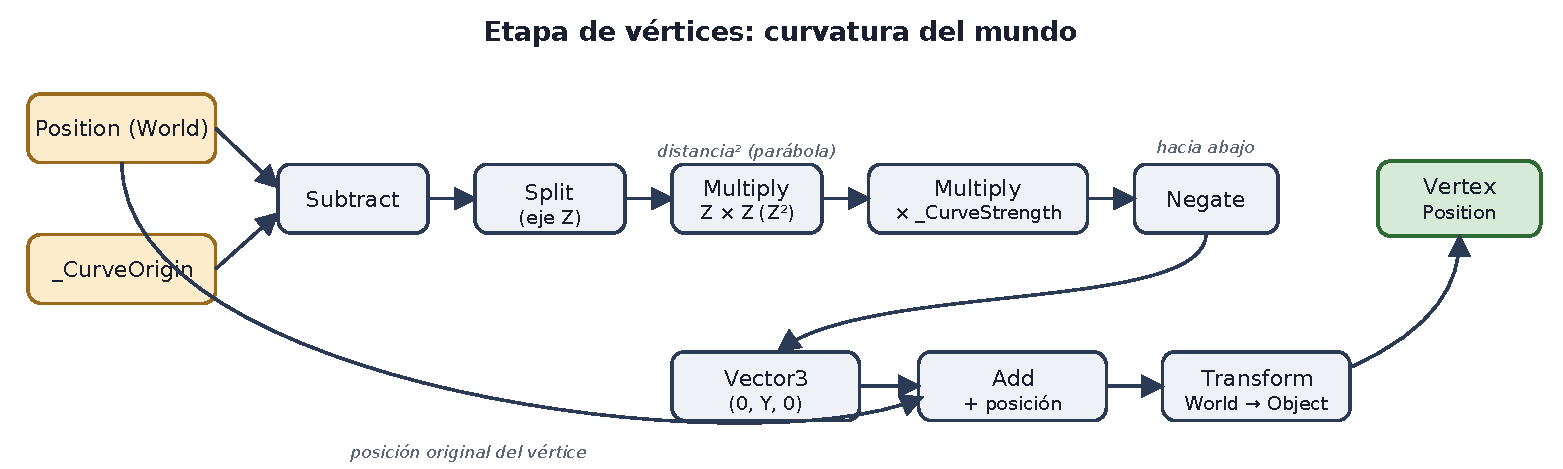
\includegraphics[width=1.2\textwidth]{esquemas/01_curvatura_vertices.pdf}
  \caption{Encadenamiento de nodos que produce la curvatura del mundo en la etapa de vértices: la posición de cada vértice se desplaza hacia abajo en función del cuadrado de su distancia al jugador, escalado por \texttt{\_CurveStrength}.}
  \label{fig:curvatura_vertices}
\end{figure}

La técnica base de curvatura no es original de este trabajo: parte de un enfoque ampliamente documentado en la comunidad de Unity, tomándose como punto de partida un tutorial divulgativo\footnote{Tutorial de referencia: «Let's learn how to make a curved Shader graph like Animal Crossing in Unity», disponible en \texttt{https://www.youtube.com/watch?v=GF0\_1-8NWBs}.} que, a su vez, se apoya en shaders previos de la comunidad. Sobre esa base, Sprout incorpora aportaciones propias que extienden el shader original ---limitado al color base--- hasta convertirlo en un sistema completo: un modelo de materiales PBR (mapa de normales, mapa metallic/smoothness empaquetado y tinte de color), una familia de cinco variantes especializadas que cubren todos los tipos de superficie del escenario (Tabla~\ref{tab:variantes_curved}) y un sistema de gestión centralizado y autogestionado.

\begin{table}[h]
  \centering
  \caption{Familia de variantes del shader de mundo curvado.}
  \label{tab:variantes_curved}
  \begin{footnotesize}
  \renewcommand{\arraystretch}{1.3}
  \begin{tabular}{p{3.2cm}p{10cm}}
    \hline
    \textbf{Variante} & \textbf{Función} \\
    \hline
    CurvedWorld & Variante completa y opaca, con sombreado PBR íntegro (color base, normales, metallic/smoothness y tinte). Referencia para superficies sólidas con detalle, como edificios y props. \\
    \hline
    CurvedWorld\_Albedo & Variante opaca simplificada que solo expone color base, para materiales planos sin texturas de detalle (por ejemplo, la floristería modelada con colores planos). \\
    \hline
    CurvedWorld\_Cutout & Añade recorte por alfa y doble cara. Imprescindible para la vegetación: las hojas son planos cuyo canal alfa define su silueta real; sin recorte se verían como rectángulos sólidos. \\
    \hline
    CurvedWorld\_Terrain & Adaptación al sistema de Terrain de Unity, basado en splatmaps, para que el suelo pintado se curve conservando su pintado. \\
    \hline
    CurvedWorld\_Water & Variante transparente con mezcla por alfa para el agua, combinando la curvatura con color translúcido, normal de oleaje y alta suavidad. \\
    \hline
  \end{tabular}
  \end{footnotesize}
\end{table}

Que la familia se componga de cinco shaders y no de uno solo no es un capricho, sino una necesidad impuesta por el motor de render: la lógica de curvatura es idéntica en todos, pero cada tipo de superficie exige un modo de render distinto ---opaco, con recorte por alfa, transparente o de terreno--- que debe declararse por separado en el shader, sin que uno solo pueda combinarlos. Por eso las variantes de la Tabla~\ref{tab:variantes_curved} comparten la deformación de vértices y se diferencian únicamente en cómo tratan la superficie: la transparencia (opaca, recortada o translúcida) y el sistema de materiales (geometría convencional o el esquema de splatmaps del Terrain). El caso de la vegetación lo ilustra la Figura~\ref{fig:material_pbr}: el recorte por alfa de la variante Cutout es lo que convierte un plano rectangular en la silueta real de una hoja.

\begin{figure}[H]
  \centering
  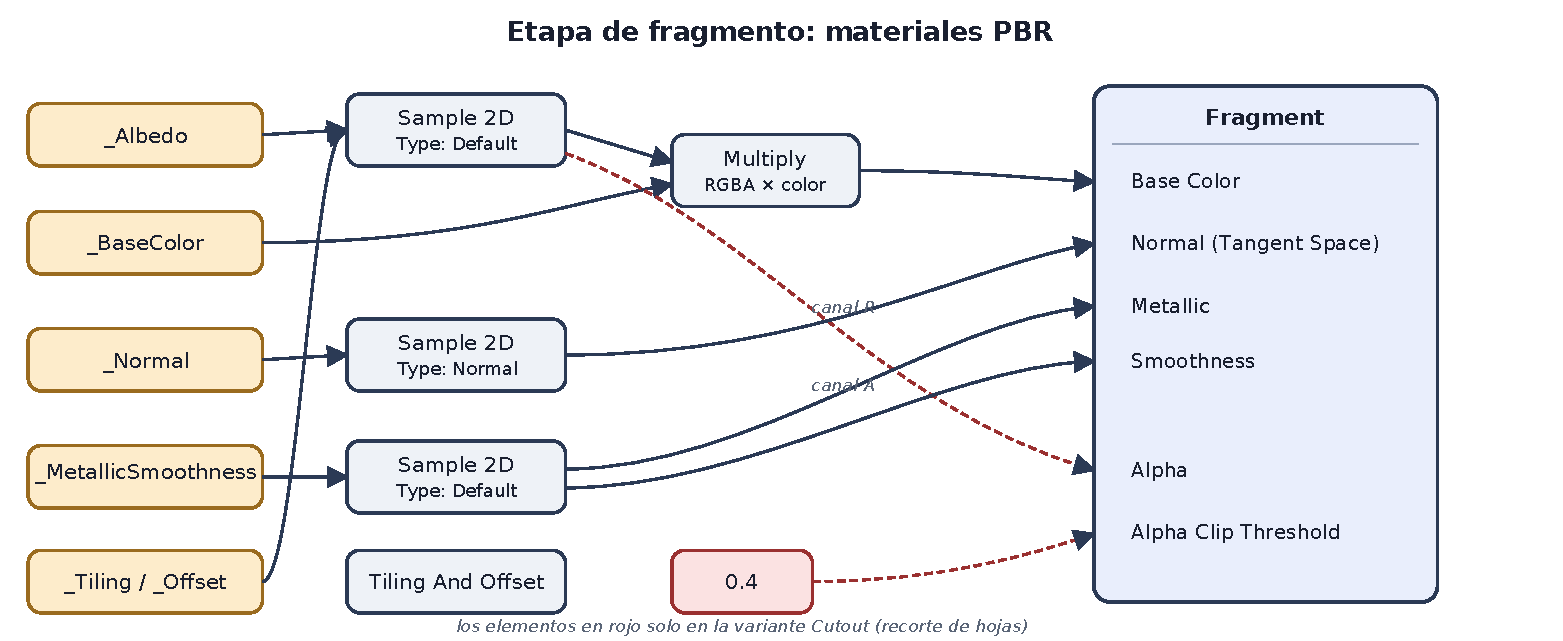
\includegraphics[width=1.2\textwidth]{esquemas/02_material_pbr.pdf}
  \caption{Encaminamiento de los materiales PBR en la etapa de fragmento: el albedo se multiplica por el tinte de color, el mapa de normales y el mapa metallic/smoothness (canales R y A) alimentan sus salidas. En rojo, los elementos exclusivos de la variante con recorte alfa para la vegetación.}
  \label{fig:material_pbr}
\end{figure}


Para que el efecto sea coherente, el centro de la curvatura debe seguir continuamente al jugador, de modo que este permanezca siempre en la cima de la pequeña esfera. De ello se encarga el componente \texttt{CurvedWorldOriginSetter}, cuyo diseño evolucionó de forma significativa durante el desarrollo, ilustrando un principio de ingeniería relevante: eliminar el mantenimiento manual propenso a errores. En una primera versión, el componente mantenía una lista de materiales asignada a mano en el inspector, que había que recordar actualizar cada vez que un objeto pasaba a usar el shader. La versión final automatiza el proceso combinando dos mecanismos: por un lado, declara \texttt{\_CurveOrigin} y \texttt{\_CurveStrength} con ámbito global y los fija una sola vez por fotograma mediante \texttt{Shader.SetGlobalVector} y \texttt{Shader.SetGlobalFloat}, de modo que alcanzan a cualquier material sin mantener referencias; por otro, recolecta al cargar la escena los materiales que usan un shader de la familia y se los aplica directamente. Como ese conjunto de materiales no cambia durante la partida, el escaneo se realiza una sola vez en ejecución; únicamente en el editor se repite de forma periódica, como comodidad de autoría para recoger los materiales que se vayan convirtiendo al shader mientras se compone la escena. El componente, marcado con \texttt{[ExecuteAlways]}, actualiza la curvatura también en el editor, permitiendo previsualizar el efecto al componer la escena. La Figura~\ref{fig:sistema_curvado} resume esta gestión centralizada.

\begin{figure}[H]
  \centering
  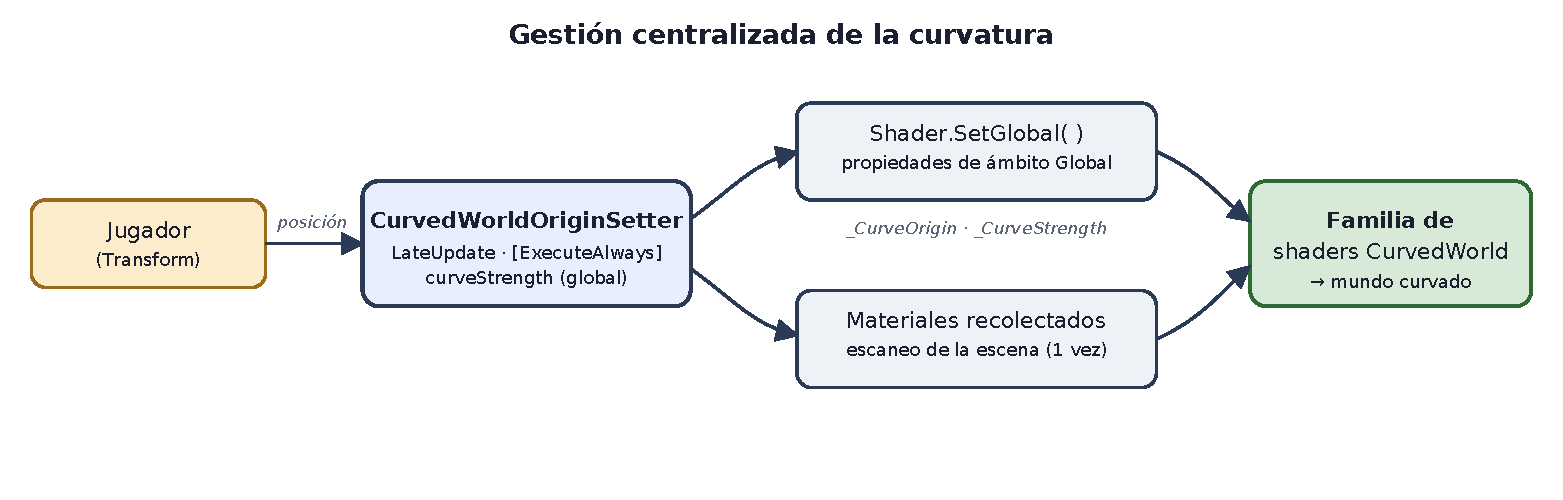
\includegraphics[width=1.2\textwidth]{esquemas/03_sistema_manager.pdf}
  \caption{Gestión centralizada de la curvatura: el componente \texttt{CurvedWorldOriginSetter} fija las propiedades globales y recolecta automáticamente los materiales de la familia de shaders, eliminando el mantenimiento manual.}
  \label{fig:sistema_curvado}
\end{figure}


\subsection{Post-procesado cozy}

Sprout combina un escenario de estilo pintado con personajes chibi de sombreado más liso. Sin un tratamiento común, esa diferencia de estilos podía leerse como una mezcla incoherente. El post-procesado se introdujo para unificar ambos registros bajo una misma atmósfera y reforzar el tono cálido y acogedor del juego, partiendo del principio de que la cohesión visual de una escena depende menos del estilo concreto de cada elemento que de que todos compartan la misma iluminación y el mismo tratamiento de color.

El efecto se construyó con el sistema de Volúmenes de URP: un \textit{Volume} global aplica a toda la escena un perfil compuesto por \textit{tonemapping} neutro (que equilibra el rango de color evitando zonas quemadas o lavadas), \textit{color adjustments} (un filtro cálido con un leve aumento de saturación y contraste), \textit{white balance} templado (que aporta la sensación de luz cálida), \textit{bloom} suave (un resplandor amable y de ensueño) y una \textit{vignette} sutil (que centra la atención en el personaje). Cada efecto responde a una intención concreta ---fijar la temperatura emocional, aportar calidez y dirigir la mirada---, y en conjunto «abrazan» a personajes y escenario bajo una misma capa de color e iluminación, de modo que el contraste de estilos deja de percibirse como un error y pasa a leerse como una elección estética. Al tratarse de un \textit{Volume} global con un perfil editable, todos los parámetros se afinan de forma centralizada y no destructiva, lo que facilitó la iteración artística.

\chapter{Evaluación}

Este capítulo documenta la evaluación del prototipo Sprout en dos niveles complementarios: playtesting con usuarios reales orientado a usabilidad y experiencia de juego  y un análisis descriptivo del comportamiento del sistema de evaluación implícita durante el playtesting . Es importante destacar desde el inicio que la validación psicométrica del sistema de evaluación implícita queda explícitamente fuera del alcance de este TFG; el presente capítulo documenta el comportamiento del sistema, no afirma su validez. La validación rigurosa contra instrumentos normativos se plantea como línea principal de trabajo futuro en el Capítulo VI.

\section{Metodología general}

La metodología de evaluación adoptada en este TFG combina dos aproximaciones complementarias. El playtesting con usuarios mide la calidad de la experiencia de juego mediante instrumentos validados (SUS, GEQ). El análisis descriptivo del sistema de evaluación implícita observa el comportamiento del perfil de creatividad durante el playtesting sin pretender validación psicométrica.

\section{Playtesting: usabilidad y experiencia}

El playtesting se realizó con una muestra de [N] participantes, reclutados por conveniencia entre el entorno cercano de la autora. Cada participante jugó una sesión completa de Sprout en condiciones controladas (auriculares, ambiente tranquilo, sin instrucciones más allá del onboarding del juego) y rellenó dos cuestionarios validados al finalizar: la System Usability Scale (Brooke, 1996) para evaluar usabilidad y el Game Experience Questionnaire (IJsselsteijn et al., 2013) para evaluar experiencia de juego. La autora estuvo presente pero no intervino salvo para resolver bloqueos técnicos.

\textcolor{gray}{\textit{[Desarrollar: tabla de participantes (N, demografía, criterios); procedimiento detallado; resultados SUS con interpretación; resultados GEQ por componente; observaciones cualitativas; ajustes derivados.]}}

\section{Análisis descriptivo del sistema de evaluación implícita}

Este apartado no constituye una validación psicométrica del sistema. Documenta de forma descriptiva el comportamiento del perfil de creatividad durante las sesiones de playtesting: distribución de las puntuaciones por dimensión, coherencia interna de los perfiles generados y capacidad del sistema para producir perfiles distinguibles entre participantes. No se compara contra ningún instrumento normativo externo ni se realizan inferencias estadísticas de validez o fiabilidad. Las limitaciones inherentes a este diseño (evaluador único, muestra pequeña, ausencia de instrumento de contraste) se reconocen explícitamente al final de la sección.

\textcolor{gray}{\textit{[Desarrollar: marco y limitaciones (repetir el matiz); recogida de datos durante playtesting; análisis descriptivo (distribución por dimensión con histogramas, perfiles individuales con radar charts, comparación cualitativa, observación de coincidencia con impresión cualitativa de la autora); limitaciones reconocidas explícitamente.]}}

\section{Discusión y ajustes derivados}

A partir de los resultados del playtesting y del análisis descriptivo, se identifican un conjunto de ajustes aplicados al prototipo y observaciones que orientan el trabajo futuro. Los ajustes se clasifican en tres categorías: correcciones de errores detectados (bugs), mejoras de usabilidad (rebalanceo de ritmo, claridad de instrucciones) y ajustes al sistema de evaluación implícita (refinamiento del system prompt del LLM evaluador).

\textcolor{gray}{\textit{[Desarrollar: ajustes técnicos, de usabilidad, y al evaluador.]}}

\chapter{Conclusiones}

\section{Conclusiones principales}

Este Trabajo Fin de Grado ha presentado el diseño e implementación de Sprout, un prototipo funcional de videojuego narrativo que evalúa de forma implícita el pensamiento divergente de la jugadora mediante conversaciones con personajes gobernados por LLM con memoria persistente. Se han alcanzado los ocho objetivos específicos planteados en la introducción: la arquitectura limpia desacoplada está implementada; el sistema de diálogo ramificado con flags y prerequisite gates funciona como base para las cuatro tramas; los cuatro NPCs tienen personalidad, voz y memoria persistente; las seis subpruebas verbales del TTCT vigente están mapeadas a momentos del juego (tres plenamente, tres integradas de forma ligera); la mecánica diferencial de la floristería emocional cierra el bucle decisión-emoción-consecuencia; y el playtesting con usuarios reales ha documentado el comportamiento descriptivo del sistema. La validación psicométrica queda como línea de continuación natural, detallada en la sección 6.3.

\section{Limitaciones reconocidas}

Una memoria académica honesta declara con claridad sus limitaciones. Las principales limitaciones de este TFG se agrupan en tres categorías: limitaciones de alcance metodológico, limitaciones técnicas y limitaciones de evaluación.

Subpruebas figurales del TTCT no implementadas (decisión deliberada de alcance, respaldada por Cramond 1994 y Ulger 2015 sobre independencia parcial verbal-figural).

Tres subpruebas verbales implementadas plenamente, tres de forma ligera (acotación de prototipo).

El sistema de evaluación implícita no ha sido validado psicométricamente; el análisis del Cap. V es descriptivo, no validatorio.

Evaluador único (LLM): no hay fiabilidad inter-evaluador establecida.

Dependencia de API externa (OpenAI): costes, latencia, privacidad de datos del jugador.

Muestra de playtesting pequeña y de conveniencia.

\section{Trabajo futuro}

Este TFG entrega un prototipo funcional y documentado, pero deja abierto un conjunto de líneas de continuación que se enumeran en orden de prioridad académica decreciente. La línea prioritaria es la validación psicométrica del sistema; el resto extiende el alcance funcional del prototipo o profundiza en aspectos específicos.

\subsection{Validación psicométrica del sistema (línea principal de continuación)}

Adquirir el TTCT-Verbal oficial vía Scholastic Testing Service, aplicarlo a una muestra ampliada de participantes que también jueguen a Sprout, y comparar las puntuaciones normativas oficiales con las que el sistema asigna internamente. Calcular fiabilidad inter-evaluador entre el LLM y evaluadores humanos entrenados según el manual del TTCT.

\subsection{Evaluación por panel humano independiente}

Sustituir o complementar al LLM evaluador con un panel de evaluadores humanos entrenados, calculando fiabilidad inter-evaluador entre humanos y entre humanos y LLM.

\subsection{Implementación de subpruebas figurales mediante mecánica de dibujo}

Integrar una mecánica de dibujo en la floristería (bocetos de ramos antes de prepararlos, planos de los inventos de Aster) que permitiría medir las tres actividades figurales del TTCT: Picture Construction, Picture Completion y Parallel Lines.

\subsection{Profundización de las subpruebas verbales ligeras}

Desarrollar contenido conversacional dedicado para las tres subpruebas integradas de forma ligera en el prototipo (Asking Questions, Guessing Causes, Guessing Consequences), elevándolas al mismo nivel de implementación que las tres plenas.

\subsection{Estudio longitudinal}

Seguimiento de participantes a lo largo del tiempo para evaluar si el desempeño en Sprout correlaciona con producción creativa real posterior, inspirado en los estudios longitudinales de Minnesota de Torrance.

\subsection{Exploración de marcos psicológicos complementarios}

ACT (Terapia de Aceptación y Compromiso) u otros marcos como capa narrativa adicional, sin pretensión de uso terapéutico.

\subsection{Ampliación de muestra y representatividad}

Pasar de muestreo por conveniencia a muestreo estratificado por edad, formación y perfil cognitivo.

%%%%%%%%%%%%%%%%%%%%%%%%%%%%%%% Bibliografía %%%%%%%%%%%%%%%%%%%%%%%%%%%%%%%

\phantomsection
\addcontentsline{toc}{chapter}{Bibliografía}

\footnotesize{
%\bibliographystyle{hispa}
\bibliographystyle{IEEEtran}
\bibliography{bibliografia}
}



% No expandir elementos para llenar toda la página
\raggedbottom
\afterpage{\blankpage}

\newpage




%%%%%%%%%%%%%%%%%%%%%%%%%%%%%%% Apéndices %%%%%%%%%%%%%%%%%%%%%%%%%%%%%%%

\appendix

\phantomsection
\addcontentsline{toc}{chapter}{Apéndices}

\mbox{}
\vfill
\begin{center}
\begin{Huge}
\textbf{Apéndices}
\end{Huge}
\end{center}
\vfill
\mbox{}
\thispagestyle{empty}

\newpage
\mbox{}
\thispagestyle{empty}
\newpage


% Primer apéndice
\chapter{System prompts completos por NPC}
\textcolor{gray}{\textit{[Incluir el prompt de sistema completo de cada uno de los cuatro personajes (Mochi, Aster, Moth y Rix): persona, conocimiento del mundo, estilo de habla y reglas obligatorias.]}}

\chapter{System prompt completo del LLM evaluador}
\textcolor{gray}{\textit{[Incluir el prompt completo del clasificador de creatividad, con el formato de salida en tubería y las instrucciones de puntuación de cada dimensión.]}}

\chapter{Diagramas UML}
\textcolor{gray}{\textit{[Incluir los diagramas: arquitectura general por capas, máquinas de estado (juego y jugador), flujo de diálogo y arquitectura del sistema de evaluación.]}}

\chapter{Árbol narrativo completo}
\textcolor{gray}{\textit{[Incluir el grafo de diálogo completo de las cuatro tramas, con nodos, puertas y flags.]}}

\chapter{Tabla de combinaciones de flores y reacciones por NPC}
\textcolor{gray}{\textit{[Incluir la tabla completa: las siete flores, las ocho combinaciones de ramo y las reacciones diferenciales de cada personaje.]}}

\chapter{Protocolo de playtesting}
\textcolor{gray}{\textit{[Incluir el guion de las sesiones de playtesting y los cuestionarios empleados (SUS, GEQ).]}}

\chapter{Resultados completos del playtesting}
\textcolor{gray}{\textit{[Incluir los resultados completos de usabilidad y experiencia, y el análisis descriptivo del perfil de creatividad.]}}

% Fin del documento
\end{document}
